图\ref{fig:classification-kernel-map}用一个二维分类例子展示特征映射$\bm{\phi}(\bm{x})=(x_1,x_1^2+x_2^2)^{\top}$。输入空间中的圆$x_1^2+x_2^2=1$，在新坐标中变成直线$\phi_2=1$；同一得分$g(\bm{x})=1-x_1^2-x_2^2$于是可以写成$g(\bm{x})=(0,-1)\bm{\phi}(\bm{x})+1$。改变的是输入的表示，原来位于圆内与圆外的样本不需要改变类别。这幅图给定了一条可行边界，用于解释几何对应，不把它当作训练后的最大间隔解。

\begin{figure}[htbp]
  \centering
  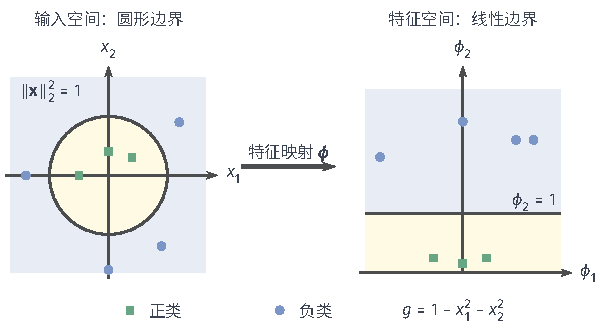
\includegraphics[width=\linewidth]{figures/03-models/01-classic-models/tikz/classification-kernel-map/figure.pdf}
  \caption{非线性边界在特征映射前后的对应，两个面板的坐标均无量纲。正类方点为$(-0.5,0)$、$(0,0.4)$、$(0.4,0.3)$，负类圆点为$(-1.4,0)$、$(0,-1.6)$、$(1.2,0.9)$、$(0.9,-1.2)$。右图逐点使用$\phi_1=x_1$、$\phi_2=x_1^2+x_2^2$；水平线$\phi_2=1$对应左图半径为1的圆。数据与边界均为教学构造。}
  \label{fig:classification-kernel-map}
\end{figure}

\subsubsection{特征映射与核技巧}
\label{sec:classic-overview-kernel-trick}
\label{sec:classification-svm-kernel-trick}

沿用\BookChapterRef{chap:functional-analysis-and-approximation}{第一卷“数学准备”的“函数空间”章}
建立的Hilbert空间与正定核。设$\bm{\phi}:\mathbb{R}^d\to\mathcal{H}$为特征映射，若能直接计算
\begin{equation}
  K(\bm{x},\bm{z})
  =\langle\bm{\phi}(\bm{x}),\bm{\phi}(\bm{z})\rangle_{\mathcal{H}},
  \label{eq:classic-overview-kernel}
\end{equation}
就可以用这个函数代替显式特征内积，而不先生成$\bm{\phi}(\bm{x})$。这种替换称为\term{核技巧}（kernel trick）。它利用的是模型计算只依赖内积的结构，不要求把无限维向量实际存入内存。

\subsubsection{正定条件与特征空间}
\label{sec:classic-overview-kernel-validity}
\label{sec:classification-svm-mercer}

相似度函数只有满足内积核的条件，才能支持上述替换。
\BookTheoremRef{thm:functional-moore-aronszajn-construction}{第一卷“数学准备”的“正定核的RKHS构造”定理}
已经从任意有限Gram矩阵的半正定性建立特征空间；取$\bm{\phi}(x)=K(\,\cdot\,,x)$即可得到式\eqref{eq:classic-overview-kernel}。
本书沿用这一命名：“正定核”允许Gram矩阵奇异，排除互异输入下的退化时才要求“严格正定核”。
核矩阵可能不可逆，具体模型必须另行规定正则化或选解方法。

需要谱坐标时，使用
\BookTheoremRef{thm:functional-mercer}{第一卷“数学准备”的“连续正定核的Mercer展开”定理}：
在紧度量输入空间、连续核及具有全支持的有限Borel测度下，核可按正特征值与特征函数展开。
一般RKHS构造不需要这些拓扑与测度条件，核技巧也不以显式求出谱展开为前提。
因而，选择核时先确认整个定义域上的正定性，再根据任务判断是否需要谱分析。

实际设计核时，不必每次重做谱分解。非负系数加权的核之和，可用特征直和构造；两个核的乘积，可用张量积特征构造，也可由Gram矩阵的Schur乘积定理验证半正定性。若一列正定核逐点收敛到有限值，则任意有限二次型的极限仍非负，极限也是正定核。这些闭包性质提供了可复用的构造规则。检查某一份训练集的Gram矩阵只能认证该有限矩阵；要使核在新样本上也合法，还需要针对整个定义域的证明或已知构造。

\subsubsection{常用核与表示选择}
\label{sec:classic-overview-common-kernels}
\label{sec:classification-svm-common-kernels}

回到$\bm{x},\bm{z}\in\mathbb{R}^d$。常用核之间的区别主要在于怎样度量接近程度、允许哪些特征交互，以及这些选择带来怎样的函数范数。表\ref{tab:classification-svm-kernels}列出五种常见形式，核尺度统一记为$\beta$，多项式次数记为$p$，避免与输入维数$d$混用。

\begin{table}[htbp]
  \centering
  \small
  \begin{tabularx}{\linewidth}{@{}>{\RaggedRight\arraybackslash}p{18mm}>{\RaggedRight\arraybackslash}X>{\RaggedRight\arraybackslash}p{27mm}@{}}
    \toprule
    名称 & $K(\bm{x},\bm{z})$ & 参数与正定性\\
    \midrule
    线性核 & $\bm{x}^{\top}\bm{z}$ & 半正定\\
    多项式核 & $(\beta\bm{x}^{\top}\bm{z}+r)^p$ & $\beta,r\ge0$，正整数$p$\\
    高斯RBF核 & $\exp(-\beta\lVert\bm{x}-\bm{z}\rVert_2^2)$ & $\beta>0$，半正定\\
    Laplacian核 & $\exp(-\beta\lVert\bm{x}-\bm{z}\rVert_1)$ & $\beta>0$，半正定\\
    Sigmoid形式 & $\tanh(\beta\bm{x}^{\top}\bm{z}+r)$ & 一般不保证半正定\\
    \bottomrule
  \end{tabularx}
  \caption{常用核函数与合法性条件。这里的“半正定”要求任意有限输入的Gram矩阵半正定；Sigmoid一行列出的是常见相似性形式，使用前仍需针对定义域与参数核验。}
  \label{tab:classification-svm-kernels}
\end{table}

\term{线性核}（linear kernel）对应$\bm{\phi}(\bm{x})=\bm{x}$，保留原始特征内积。对于线性预测，训练样本的核展开可以聚合为一个权重向量，使用时不必逐一访问这些样本。是否需要额外的非线性交互，应通过任务与验证数据判断；输入维数高本身既不保证线性结构足够，也不意味着非线性核必然更好。

\term{多项式核}（polynomial kernel）把有限阶交互隐式加入模型。以$d=2$、$\beta=1$、$r=0$、$p=2$为例，
\[
  \begin{aligned}
    (\bm{x}^{\top}\bm{z})^2
      &=x_1^2z_1^2+2x_1x_2z_1z_2+x_2^2z_2^2,\\
    \bm{\phi}(\bm{x})
      &=(x_1^2,\sqrt2\,x_1x_2,x_2^2)^{\top}.
  \end{aligned}
\]
交叉项前的$\sqrt2$使特征内积准确等于核值。一般地，令多重指标$\bm{a}=(a_1,\ldots,a_d)$满足$|\bm{a}|=\sum_j a_j=p$，并记$\bm{x}^{\bm{a}}=\prod_j x_j^{a_j}$、$\bm{a}!=\prod_j a_j!$。多项式展开为
\[
  (\bm{x}^{\top}\bm{z})^p
  =\sum_{|\bm{a}|=p}\frac{p!}{\bm{a}!}
     \bm{x}^{\bm{a}}\bm{z}^{\bm{a}}.
\]
所以齐次$p$次核可以使用$\binom{d+p-1}{p}$个单项式坐标；当$\beta>0,r>0$时，非齐次核包括$0$至$p$次项，一种完整单项式表示的维数是$\binom{d+p}{p}$。这些是特征数量，不是样本数量；计算一个核值通常只需一次$d$维内积和幂运算，节省的是显式特征展开成本，完整优化仍要另计。

\term{高斯径向基核}（Gaussian radial basis function kernel，Gaussian RBF kernel）根据欧氏距离赋予局部相似性。其无限维特征可以由指数级数直接看出：
\begin{equation}
  \begin{aligned}
    K(\bm{x},\bm{z})
      ={}&e^{-\beta\lVert\bm{x}\rVert_2^2}
          e^{-\beta\lVert\bm{z}\rVert_2^2}\\
       &\cdot\sum_{p=0}^{\infty}
          \frac{(2\beta)^p}{p!}
          (\bm{x}^{\top}\bm{z})^p.
  \end{aligned}
  \label{eq:classification-svm-rbf-expansion}
\end{equation}
每一阶多项式核都是半正定的，系数非负，两个单点因子可以吸收到特征中；级数逐点收敛，因而也给出了高斯核合法性的证明。把每一阶的单项式展开合并，坐标可写成
\[
  \phi_{\bm{a}}(\bm{x})
  =e^{-\beta\lVert\bm{x}\rVert_2^2}
     \sqrt{\frac{(2\beta)^{|\bm{a}|}}{\bm{a}!}}\,
     \bm{x}^{\bm{a}},
  \qquad \bm{a}\in\mathbb{N}_0^d.
\]
这里$\mathbb{N}_0$为非负整数集合，所有坐标平方之和等于$K(\bm{x},\bm{x})=1$。在整个$\mathbb{R}^d$上，这个核具有无限秩；限制到一批有限训练点以后，实际使用的Gram矩阵仍是$n\times n$。

参数$\beta$控制相似性随距离衰减的速度，也常写成$\beta=1/(2\sigma^2)$。较大$\beta$使不同训练点之间的相似性迅速减小，模型能够形成更局部的变化；较小$\beta$使作用范围更宽。对互异有限输入，高斯Gram矩阵严格正定，因此在不约束范数时，线性方程$\bm{K}\bm{a}=\bm{y}$允许核展开插值给定标签。然而所需系数与函数范数可能很大；固定范数、固定正则化强度或有重复输入且标签冲突时，都不能由“无限维”推出任意插值，更不能由插值推出泛化良好。

\term{Laplacian核}（Laplacian kernel）使用$L^1$距离，且可以分解成各坐标上的乘积：
\[
  \exp(-\beta\lVert\bm{x}-\bm{z}\rVert_1)
  =\prod_{j=1}^d\exp(-\beta|x_j-z_j|).
\]
一维形式的半正定性可由积分特征表示验证：
\[
  e^{-\beta|t|}
  =\int_{\mathbb{R}}e^{\mathrm{i}\omega t}
      \frac{\beta}{\pi(\beta^2+\omega^2)}\,\mathrm{d}\omega.
\]
其中$\mathrm{i}$为虚数单位。对任意有限个输入$x_j$和实系数$a_j$，将有限求和移入积分可得
\[
  \begin{aligned}
    &\sum_{j,k}a_j a_k e^{-\beta|x_j-x_k|}\\
    &\quad=\int_{\mathbb{R}}
      \left|\sum_j a_j e^{\mathrm{i}\omega x_j}\right|^2
      \frac{\beta}{\pi(\beta^2+\omega^2)}\,\mathrm{d}\omega
      \ge0.
  \end{aligned}
\]
多维形式再由核的乘积闭包得到。Laplacian核在零距离附近的变化方式与高斯核不同，可以作为直方图或稀疏特征上的另一种距离选择，但哪一种更适合仍取决于尺度、表示与验证结果。

常称为\term{Sigmoid核}（sigmoid kernel）的形式将内积送入双曲正切函数，形态上接近一个具有非线性激活的神经元，却不自动具有内积核的性质。甚至$\beta=1,r=0$也不能在整个实数域上保证半正定：对$x_1=1,x_2=2$，二阶Gram行列式为
\[
  \tanh(1)\tanh(4)-\tanh(2)^2
  \approx-0.1683<0.
\]
因此“参数取正”并不足以保证合法。某个有限数据集上矩阵没有负特征值，只说明当前矩阵通过检查；若要保留依赖内积核的几何与优化解释，应选用在目标定义域上已确认半正定的核。

对字符串、图与树，核技巧同样适用。\term{字符串核}（string kernel）可以计数共同的子串或子序列，\term{图核}（graph kernel）可以比较局部子结构，\term{树核}（tree kernel）可以比较子树模式。若将每种模式的出现次数作为一个坐标，两对象的模式计数内积就给出了直接的正定构造；动态规划或结构化计数有时能避免把全部坐标显式列出。这样的\term{结构化核}（structured kernel）把输入的组合结构用于相似性计算，适用于序列分析、分子图或句法树等场景，并通过可验证的特征内积保留核方法的几何与优化性质。

\subsubsection{核矩阵的使用与中心化}
\label{sec:classic-overview-kernel-matrix}

在$n$个训练输入上，核矩阵的元素为$\bm{K}_{i,j}=K(\bm{x}_i,\bm{x}_j)$。完整存储需要$O(n^2)$空间和$O(n^2)$次核计算；显式特征可以很大甚至无限维，并不意味着样本之间的计算也消失了。缓存、稀疏化或低秩近似会改变实现成本，近似误差仍须与具体任务一起评价。

有些方法要求在特征空间中先减去训练均值。令$\bm{1}\in\mathbb{R}^{n}$为全一向量、$\bm{I}_n$为单位矩阵，中心化矩阵及中心化核矩阵为
\begin{equation}
  \bm{H}=\bm{I}_n-\frac1n\bm{1}\bm{1}^{\top},
  \qquad \bm{K}_{\mathrm{c}}=\bm{H}\bm{K}\bm{H}.
  \label{eq:classic-overview-kernel-centering}
\end{equation}
左乘$\bm{H}$减去各列均值，右乘$\bm{H}$减去各行均值；展开双边乘积时，还要加回原核矩阵的整体均值。结果等于中心化特征的内积矩阵。只对原始输入作中心化，一般不能代替非线性特征中心化。新样本也应使用训练特征的均值，不能重新用测试数据定义中心。中心化是否必要由具体目标决定，例如核PCA需要它，高斯过程的协方差建模则不因此一律先作这种变换。
